\section{Method and Setup}
\label{sec:method}

\begin{figure*}[t]
\centering
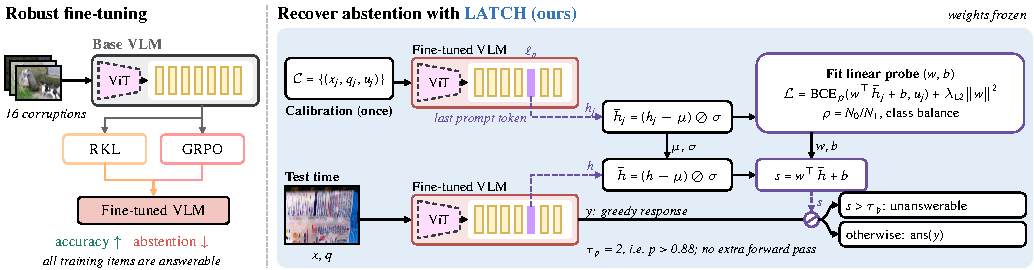
\includegraphics[width=\textwidth]{figures/method.pdf}
\caption{\textbf{Overview.} Robust fine-tuning (RKL or GRPO) raises accuracy but lowers
abstention. LATCH restores it with frozen weights: a latent check, fitted once per model on
a calibration set $\mathcal{C}$, replaces the answer by ``unanswerable'' when the probe
logit $s$ exceeds $\tau_{\mathrm{p}}$ ($P(\text{unanswerable}) > 0.88$). $(x, q)$: image and
question; $y$: response; $u$: answerability label ($u = 1$: unanswerable);
$\mathrm{BCE}_\rho$: binary cross-entropy that weights the $N_1$ unanswerable calibration
items by $\rho = N_0/N_1$, with $N_0$ answerable items. The two baselines are drawn in \cref{fig:supp_retrain,fig:supp_steer}.}
\label{fig:method}
\end{figure*}

\subsection{Problem formulation}
\label{sec:problem}

\paragraph{Visual question answering with abstention.}
Each item of a dataset $\mathcal{D}$ has an image $x \in \mathbb{R}^{H \times W \times 3}$, a question $q$, and a label $u \in \{0, 1\}$: $u = 0$ if the image shows the answer, and $u = 1$ if it does not (it is too degraded, or withheld). An answerable item has a gold
answer $a^\star$ and a set $\mathcal{A}(x, q)$ of accepted answers: the annotators'
answers, or $\{a^\star\}$ on GQA. A VLM is a policy $\pi$ that writes a response
$y \in \mathcal{V}^T$ of $T$ tokens, $y_t \sim \pi(\cdot \mid y_{<t}, x, q)$, ending in one
\texttt{<answer>} block; the answer parsed from this block is $\mathrm{ans}(y)$. The refusal
indicator $\mathrm{ref}(y) \in \{0, 1\}$ is $1$ if $\mathrm{ans}(y)$ contains a refusal
phrase such as ``unanswerable'' (full list in \cref{sec:setup}). As in selective
prediction~\cite{geifman2017selective}, we score answering and abstaining separately. With
$y$ the response from $\pi$ and $\mathbb{E}_{\mathcal{D}}$ the average over a set
$\mathcal{D}$ of items, the accuracy ($\mathrm{Acc}$; $\uparrow$), correct-refusal rate
($\mathrm{CR}$; $\uparrow$) and unnecessary-refusal rate ($\mathrm{UR}$; $\downarrow$) are
\begin{align}
\mathrm{Acc}(\pi;\mathcal{D}) &= \mathbb{E}_{\mathcal{D}}\,
  \mathds{1}\!\left[\mathrm{ans}(y) \in \mathcal{A}(x,q)\right], \label{eq:acc}\\
\mathrm{CR}(\pi;\mathcal{D}) &= \mathbb{E}_{\mathcal{D}}\!\left[\mathrm{ref}(y) \mid u = 1\right],
  \label{eq:cr}\\
\mathrm{UR}(\pi;\mathcal{D}) &= \mathbb{E}_{\mathcal{D}}\!\left[\mathrm{ref}(y) \mid u = 0\right].
  \label{eq:ur}
\end{align}

\paragraph{Corruption-robust fine-tuning.}
VLMs lose accuracy on degraded images~\cite{usama2025analysing}, so a common remedy is to fine-tune them on degraded images. A corrupted image $\tilde{x}$ is $x$ with one corruption applied, such as fog or blur. Robust fine-tuning starts from a base VLM $\pi_0$, trains on a set $\mathcal{D}_{\mathrm{train}}$ of items $(x, \tilde{x}, q, a^\star)$ to raise accuracy on $\tilde{x}$, and returns $\pi_\theta$, the same model with parameters $\theta$. This training is label-preserving: a corrupted image keeps the label of its clean image~\cite{hendrycks2020augmix,liu2023softaug,he2026videoreasoningmodelsready}, even when strong corruption removes the information the label depends on~\cite{liu2023softaug}. Every training item is therefore answerable ($u = 0$), so $\mathrm{CR}$ never enters the training objective.

We evaluate models on two sets. The answerable set $\mathcal{D}_{\mathrm{A}}$ ($u = 0$) holds questions on clean images, on corrupted copies of them, and on real photographs that still show the answer; $\mathcal{D}_{\mathrm{A}}^{\mathrm{C}} \subset \mathcal{D}_{\mathrm{A}}$ is its corrupted part. The unanswerable set $\mathcal{D}_{\mathrm{U}}$ ($u = 1$) contains real photographs too degraded to answer and questions asked without their images (\cref{sec:setup}). Compared with $\pi_0$, fine-tuning raises accuracy on corrupted images, $\mathrm{Acc}(\pi_\theta;\mathcal{D}_{\mathrm{A}}^{\mathrm{C}})$, but lowers the rate of correct refusals, $\mathrm{CR}(\pi_\theta;\mathcal{D}_{\mathrm{U}})$ (\cref{sec:regression}).


% \paragraph{Hidden states and probes.}
% For a model $\pi$ and decoder layer $\ell$, let $h^{(\ell)}_{\pi}(x,q) \in \mathbb{R}^{d}$
% be the hidden state at the last prompt token, just before the response begins, where $d$ is
% the hidden width. A linear probe $(w, b) \in \mathbb{R}^{d} \times \mathbb{R}$ predicts $u$
% from $h^{(\ell)}_{\pi}$ (\cref{eq:probe}). Its AUROC on held-out items,
% $\mathrm{AUROC}_\ell(\pi) \in [0,1]$ with $0.5$ at chance, measures how well layer $\ell$
% of $\pi$ encodes answerability.

\begin{tcolorbox}[enhanced, breakable, colback=probback, colframe=probframe, arc=2mm,
  boxrule=0.8pt, left=5pt, right=5pt, top=4pt, bottom=4pt]
\textbf{Problem Description.} Given the base model $\pi_0$, its fine-tuned version
$\pi_\theta$, and the evaluation sets $\mathcal{D}_{\mathrm{A}}$ and $\mathcal{D}_{\mathrm{U}}$, \uline{our goal is to recover abstention without giving up the robustness gains}: find an intervention $g$, either retraining $\pi_0$ on modified data or an inference-time rule applied to $\pi_\theta$, whose model $\pi'$, evaluated on the same items, prompt and
decoding as $\pi_\theta$, solves
\begin{equation}
\begin{aligned}
\max_{g}\ \ & \mathrm{CR}(\pi';\mathcal{D}_{\mathrm{U}}) \\
\text{s.t.}\ \ & \mathrm{Acc}(\pi';\mathcal{D}_{\mathrm{A}}^{\mathrm{C}}) \ge
  \mathrm{Acc}(\pi_\theta;\mathcal{D}_{\mathrm{A}}^{\mathrm{C}}) - \Delta_{\mathrm{acc}}, \\
& \mathrm{UR}(\pi';\mathcal{D}_{\mathrm{A}}) \le \mathrm{UR}_{\max},
\end{aligned}
\label{eq:recover}
\end{equation}
where $\Delta_{\mathrm{acc}}$ is the tolerated loss of corrupted accuracy and
$\mathrm{UR}_{\max}$ the tolerated unnecessary-refusal rate (RQ3).
\end{tcolorbox}

Prior work either fine-tunes VLMs for corruption robustness and reports accuracy
alone~\cite{he2026videoreasoningmodelsready,tang2026robustr1,liu2026roma}, or studies and adds abstention in models as released~\cite{miyai2024upd,zhu2025mohobench,madhusudhan2026knowing,pramono2026trapsbench,he2026knowing,vardi2025clipup}; to our knowledge, recovering abstention after robustness fine-tuning, without losing its gains, has not been posed (\cref{sec:related}). The problem arises wherever a model is fine-tuned on answerable-only data ($u = 0$ throughout $\mathcal{D}_{\mathrm{train}}$) and deployed where unanswerable inputs occur, as in assistive, driving and medical imaging. It is hard for two reasons: the regression is invisible during training and on accuracy benchmarks, since $\mathrm{CR}$ enters neither the training objective nor $\mathrm{Acc}$; and both constraints of \cref{eq:recover} pull against the objective, because a fix that refuses more can give back corrupted accuracy or
refuse answerable questions.

Given a base VLM $\pi_0$, we make it robust to corruptions, locate what this does to its
abstention, and then repair it, which solves \cref{eq:recover}, in three
steps:
\ding{182}~We fine-tune $\pi_0$ on corrupted images with RKL or GRPO, which gives
$\pi_\theta$ (\cref{sec:method-ft}).
\ding{183}~We locate where abstention is lost, which tells us what an intervention can use:
a linear probe reads $u$ from the model's hidden state (\cref{eq:diagnose}), and a
reasoning transplant tests whether $\pi_\theta$ drops the refusal in its reasoning or in
its answer (\cref{sec:method-diagnose}).
\ding{184}~We recover abstention (\cref{eq:recover}) with LATCH, a latent check that turns
the probe of step~\ding{183} into a refusal rule (\cref{sec:method-remedies}).

\subsection{Corruption-robust fine-tuning}
\label{sec:method-ft}

Both recipes train $\pi_\theta$ on its own sampled responses to the corrupted image
$\tilde{x}$. They differ only in what scores those responses: a teacher's token
distribution for RKL, a verifiable reward for GRPO.

\paragraph{On-policy reverse-KL distillation (RKL).}
Knowledge distillation trains a student to match a teacher's output distribution instead
of hard labels~\cite{hinton2015distilling}. On-policy
distillation~\cite{agarwal2024onpolicydistillationlanguagemodels} lets the student sample
its own responses and has the teacher score every token of them, so the student is
corrected on the prefixes it reaches itself rather than on the teacher's (exposure bias).
Here the student $\pi_\theta$ sees $\tilde{x}$, and a frozen teacher
$\pi_{\mathrm{teach}}$, a larger model of the same family, sees the clean image $x$. For
each question we sample $N_{\mathrm{roll}} = 2$ responses
$y \sim \pi_\theta(\cdot \mid \tilde{x}, q)$ and minimize the reverse KL at every position
$t \in \{1,\dots,T\}$:
\begin{equation}
\begin{aligned}
\mathcal{L}_{\mathrm{RKL}}(\theta) = \mathbb{E}\Big[\textstyle\sum_{t=1}^{T}
\mathrm{KL}\big(&\pi_\theta(\cdot \mid y_{<t}, \tilde{x}, q) \\
\,\big\|\,&\pi_{\mathrm{teach}}(\cdot \mid y_{<t}, x, q)\big)\Big],
\end{aligned}
\label{eq:rkl}
\end{equation}
with the expectation over $(x, \tilde{x}, q) \sim \mathcal{D}_{\mathrm{train}}$ and
$y \sim \pi_\theta(\cdot \mid \tilde{x}, q)$. Each term measures how far the student's
next-token distribution on $\tilde{x}$ is from the teacher's on $x$, after a prefix the
student wrote itself. Reverse KL is mode-seeking: the student concentrates on the
teacher's dominant continuations rather than covering all of them~\cite{gu2024minillm}. We
estimate each term from the sampled token, as a policy gradient with advantage
$A_t = \log \pi_{\mathrm{teach}}(y_t \mid \cdot) - \log \pi_\theta(y_t \mid \cdot)$.
RKL needs
no gold answers, only teacher forward passes.

\paragraph{Group Relative Policy Optimization (GRPO).}
GRPO~\cite{shao2024deepseekmath} replaces the teacher with a verifiable reward and PPO's
value network with a group baseline, and it sees only $\tilde{x}$. For each question it
samples $G = 8$ responses $y^{(i)} \sim \pi_{\theta_{\mathrm{old}}}(\cdot \mid \tilde{x}, q)$,
$i \in \{1,\dots,G\}$, from the policy before the update, and scores each as
\begin{equation}
r_i = \mathds{1}\!\left[\mathrm{fmt}_i \wedge \mathrm{ans}(y^{(i)}) = a^\star\right]
      + w_{\mathrm{fmt}}\, \mathrm{fmt}_i,
\label{eq:reward}
\end{equation}
where $\mathrm{fmt}_i \in \{0,1\}$ is $1$ if $y^{(i)}$ has exactly one \texttt{<answer>}
block and ends right after it, $w_{\mathrm{fmt}} = 0.1$, and $a^\star$ is the GQA gold
answer (exact match). For
example, a well-formed response with the gold answer earns $r_i = 1.1$, a well-formed wrong
answer $0.1$, and a response cut off before its \texttt{<answer>} block $0$. Advantages are
standardized within the group,
\begin{equation}
\hat{A}_i = \frac{r_i - \mathrm{mean}(r)}{\mathrm{std}(r) + \epsilon_{\mathrm{std}}},
\label{eq:adv}
\end{equation}
and the policy maximizes the clipped surrogate with a KL anchor to the base model:
\begin{equation}
\begin{aligned}
\mathcal{J}_{\mathrm{GRPO}}(\theta) = \mathbb{E}\Big[
&\tfrac{1}{\sum_i |y^{(i)}|}\textstyle\sum_{i,t}
\min\!\big(\rho_{i,t}\hat{A}_i,\, \bar\rho_{i,t}\hat{A}_i\big) \\
&- \beta\,\mathrm{KL}(\pi_\theta \,\|\, \pi_0)\Big].
\end{aligned}
\label{eq:grpo}
\end{equation}
Here $i$ ranges over the group and $t$ over the tokens of $y^{(i)}$,
$\rho_{i,t} = \pi_\theta(y^{(i)}_t \mid \tilde{x}, q, y^{(i)}_{<t}) /
\pi_{\theta_{\mathrm{old}}}(y^{(i)}_t \mid \tilde{x}, q, y^{(i)}_{<t})$ is the ratio of the
current to the sampling policy, $\bar\rho_{i,t} = \mathrm{clip}(\rho_{i,t},
1 - \epsilon_{\mathrm{clip}}, 1 + \epsilon_{\mathrm{clip}})$, $\epsilon_{\mathrm{clip}} = 0.2$,
$\epsilon_{\mathrm{std}} = 10^{-6}$ and $\beta = 0.04$; the token mean is taken over all
groups of an optimizer step. Because every training item has $u = 0$, a well-formed refusal
scores like any wrong answer ($r_i = 0.1$), and its advantage is negative whenever another
response in its group is correct: no term of \cref{eq:reward,eq:grpo} ever rewards
abstaining.

\subsection{Locating the loss}
\label{sec:method-diagnose}

We next ask where the refusal is lost: in the representation of answerability, in the
reasoning, or in the answer.

\paragraph{Answerability probe.}
For a model $\pi$ and decoder layer $\ell \in \{1,\dots,L\}$, one prefill gives the
residual-stream state $h^{(\ell)}_{\pi}(x,q) \in \mathbb{R}^{d}$ at the last prompt token,
the position just before the response begins. We standardize each of its $d$ features,
$\bar{h} = (h^{(\ell)}_{\pi}(x,q) - \mu) \oslash \sigma$ with $\oslash$ element-wise
division, by the mean $\mu$ and standard deviation $\sigma$ over a labeled calibration set
$\mathcal{C} = \{(x_j, q_j, u_j)\}_{j=1}^{N_{\mathcal{C}}}$, so that one L2 strength
penalizes all features on the same scale. We then fit a class-balanced, L2-regularized
logistic regression
\begin{equation}
p_\ell(u = 1 \mid x, q) = \mathrm{sigmoid}\big(w^\top \bar{h} + b\big),
\label{eq:probe}
\end{equation}
one per model and layer, on that model's own states; class balancing offsets the unequal
class sizes of $\mathcal{C}$. The AUROC of the logit $w^\top \bar{h} + b$ on held-out
items, $\mathrm{AUROC}_\ell(\pi) \in [0,1]$, measures how well layer $\ell$ of $\pi$ encodes
$u$; the same probe fitted on shuffled labels gives its chance floor. We say the probe
\emph{flags} an input when the logit exceeds $0$. Because the probe reads the state from
which the response starts, it tests whether
\begin{equation}
\begin{gathered}
\mathrm{AUROC}_\ell(\pi_\theta) \approx \mathrm{AUROC}_\ell(\pi_0) \\
\text{while}\ \
\mathrm{CR}(\pi_\theta;\mathcal{D}_{\mathrm{U}}) < \mathrm{CR}(\pi_0;\mathcal{D}_{\mathrm{U}}),
\end{gathered}
\label{eq:diagnose}
\end{equation}
\ie whether $\pi_\theta$ still encodes that the input is unanswerable when it begins to
answer. If so, the failure is behavioral rather than representational (RQ1), and an
intervention can use the signal that survives.

\paragraph{Reasoning transplant.}
A refusal can be lost in the reasoning, which never concludes that the image is
insufficient, or in the answer, which ignores reasoning that does. For example, on a blurry VizWiz photo
of jellybeans the RKL response lists flavors it cannot see, a reasoning-side failure, while
on the removed image of \cref{fig:teaser} the GRPO response states that ``there is no
visible number on the jersey'' and still gives $\mathrm{ans}(y) = $ ``3'', an answer-side failure. To separate the two at scale, we
take the unanswerable items that $\pi_\theta$ answered and $\pi_0$ refused, prefill
$\pi_\theta$ with $(x, q)$ followed by $\pi_0$'s response up to and including
\texttt{<answer>}, and record whether $\pi_\theta$'s answer is a refusal. If $\pi_\theta$
now refuses, its answer step follows a ``can't-tell'' chain, so its failure is that its own
reasoning never produces one; if it still answers, its answer step overrides the reasoning. Further details on this is given in \cref{sec:rq2}

\subsection{Recovering abstention}
\label{sec:method-remedies}

We finally ask how to bring the refusal back without giving up the gains of
step~\ding{182}. LATCH is an intervention $g$ in \cref{eq:recover} that keeps $\theta$ fixed
and acts at inference. We compare it with two baselines: retraining $\pi_0$ from scratch
with the same recipe and budget on a mix in which $10\%$ of the questions are unanswerable
(\cref{sec:supp_train_data}), and activation steering, which moves the hidden states of
$\pi_\theta$ toward those of $\pi_0$ while it writes (\cref{sec:supp_steer_method}).

\begin{algorithm}[t]
\caption{\textbf{LATCH: one linear read of the prompt replaces an answer by a
refusal.} Lines 1--3 run once per model; lines 4--8 add no forward pass.}
\label{alg:latch}
\begin{algorithmic}[1]
\Require model $\pi$, layer $\ell_{\mathrm{p}}$, calibration set
  $\mathcal{C} = \{(x_j, q_j, u_j)\}$, L2 strength $\lambda_{\mathrm{L2}}$, cutoff
  $\tau_{\mathrm{p}}$
\State $h_j \gets h^{(\ell_{\mathrm{p}})}_{\pi}(x_j, q_j)$ for every
  $j$ \Comment{prefill only}
\State $\mu, \sigma \gets$ mean and std.\ of $\{h_j\}$;
  $\bar{h}_j \gets (h_j - \mu) \oslash \sigma$
\State $(w, b) \gets$ fit \cref{eq:probe} to $\{(\bar{h}_j, u_j)\}$, class-balanced, L2
  strength $\lambda_{\mathrm{L2}}$
\State On a test input $(x, q)$: prefill and read
  $\bar{h} \gets (h^{(\ell_{\mathrm{p}})}_{\pi}(x, q) - \mu) \oslash \sigma$
\State $y \gets$ greedy response of $\pi(\cdot \mid x, q)$ \Comment{reuses the prefill}
\If{$w^\top \bar{h} + b > \tau_{\mathrm{p}}$}
  \State \Return ``unanswerable''
\EndIf
\State \Return $\mathrm{ans}(y)$
\end{algorithmic}
\end{algorithm}

\paragraph{LATCH (LATent CHeck).}
The probe of \cref{sec:method-diagnose} still reads $u$ after fine-tuning (\cref{sec:rq1}),
so LATCH acts on it directly (\cref{fig:method,alg:latch}). Lines~1--3 fit that probe at a
single layer $\ell_{\mathrm{p}}$, once per model and on that model's own states. Lines~4--5
run the model unchanged and reuse its prefill for the probe. Lines~6--7 replace the answer by
a refusal when the probe logit exceeds $\tau_{\mathrm{p}}$; line~8 otherwise returns the
model's own answer. Thus LATCH changes $\mathrm{ans}(y)$ only on inputs it flags, so
the robustness gained on answerable inputs is kept wherever it does not fire, and
$\tau_{\mathrm{p}}$ sets the trade-off between $\mathrm{CR}$ and $\mathrm{UR}$ in
\cref{eq:recover}.

\subsection{Experimental setup}
\label{sec:setup}

\paragraph{Metrics.}
We report the three quantities of \cref{sec:problem}, all in \%. A response is a
refusal, $\mathrm{ref}(y) = 1$, if $\mathrm{ans}(y)$ contains ``unanswerable'',
``cannot'', ``unable'', ``not possible'', ``impossible'', ``no image'', ``not visible'',
``not provided'' or ``not determin''. \emph{Accuracy} (\cref{eq:acc}) is measured on
clean and on corrupted images: training uses corrupted images, so clean accuracy checks
that the model has not lost what it could already do. A prediction is correct if
$\mathrm{ans}(y)$ matches the answer (GQA) or any of the ten annotator answers (TextVQA,
VQAv2, VizWiz), \emph{and} is not a refusal. The second condition matters because some
annotators answer ``unanswerable'' even on questions labeled answerable ($46\%$ of
answerable VizWiz questions, $10\%$ of TextVQA questions); without it, a remedy that
refuses more would also appear to answer better. \emph{Correct refusals} ($\mathrm{CR}$,
\cref{eq:cr}; higher is better) are measured on unanswerable VizWiz questions, and
\emph{no-image refusals} are the same rate on TextVQA, GQA and VQAv2 questions asked
with the image withheld (mean of the three), where any answer is a guess from language
priors. \emph{Unnecessary refusals} ($\mathrm{UR}$, \cref{eq:ur}; lower is better) are
measured on answerable VizWiz questions. We also report \emph{answerable} and
\emph{unanswerable accuracy} on VizWiz; because VizWiz has ten annotator answers per
question, unanswerable accuracy also credits non-refusal answers that some annotators
gave.

\paragraph{Benchmarks.}

\begin{figure*}[t]
\centering
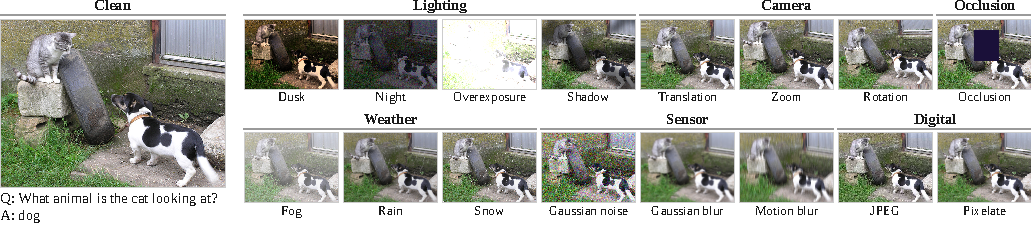
\includegraphics[width=\textwidth]{figures/fig_gqa_corruptions.pdf}
\caption{\textbf{Training data: one GQA question under all $16$ corruptions.} A real
question from our GQA training set, shown clean and under every corruption style at
severity $4$, the severity used for training, grouped into six families (lighting,
camera, occlusion, weather, sensor, digital). Each training question receives one
style, assigned uniformly ($1{,}875$ of the $30{,}000$ questions per style); the
question and answer are unchanged.}
\label{fig:gqa_corruptions}
\end{figure*}

We use one short name per evaluation set (\cref{tab:data}).
\textbf{TextVQA-C}, \textbf{GQA-C} and \textbf{VQAv2-C} are TextVQA, GQA and VQAv2 corrupted
with the standard ImageNet-C engine~\cite{hendrycks2019imagenetc}: $19$ types in $4$ groups
(noise, blur, weather, digital) at severities $1$--$5$; \textbf{TextVQA}, \textbf{GQA} and
\textbf{VQAv2} denote the same questions on clean images. \textbf{VizWiz}~\cite{gurari2018vizwiz}
is not corrupted synthetically: its $4{,}319$ validation photographs ($2{,}934$ answerable,
$1{,}385$ unanswerable) are blurry, badly framed or dark from how blind users captured them,
and it is our only source of real degradation and real unanswerable questions.
\textbf{No-image} is TextVQA, GQA and VQAv2 with the image withheld.
The comparison is fair in three ways. Every model is evaluated on the same rendered
images, because each corruption is seeded per question. Training and evaluation use
different corruption engines by design: only $8$ of the $19$ evaluation types have a
training counterpart, so the other $11$ (${\sim}58\%$ of corrupted questions) are unseen by
every model. All models are decoded greedily with the same $768$-token limit, and the
retrained models use the same number of optimization steps as the runs they are compared
with. All the models and their retrained versions were evaluated using the same prompt. We only add a single line to the prompt, "If the image does not contain enough information to answer, the answer is unanswerable.", when we are evaluating on the VizWiz dataset or on the dataset without any image.


\begin{table}[tb]
\centering
\caption{\textbf{Training and evaluation deliberately use different corruption engines.}
\#Q: number of questions.}
\label{tab:data}
\footnotesize
\setlength{\tabcolsep}{3pt}
\begin{tabular}{@{}llrl@{}}
\toprule
Set & Source & \#Q & Role / corruption \\
\midrule
GQA train      & GQA tr.\ bal.  & 30{,}000 & train; 16 types \\
Destroyed-GQA  & GQA tr.\ bal.  & 3{,}334  & 10\% mix; 7 types \\
TextVQA-C      & TextVQA val    & 5{,}000  & eval; ImageNet-C \\
GQA-C          & GQA testdev    & 12{,}578 & eval; ImageNet-C \\
VQAv2-C        & VQAv2 val      & 5{,}000  & eval; ImageNet-C \\
VizWiz         & VizWiz val     & 4{,}319  & eval; real (2934/1385) \\
Probe calib.   & VizWiz train   & 1{,}901  & probe; 1101 unans./800 ans. \\
Steering calib.& train splits   & ---      & vectors; all 4 eval sources \\
\bottomrule
\end{tabular}
\end{table}

\paragraph{Models and training.}
We study three 4B-parameter instruction-tuned VLMs: Qwen3-VL-4B-Instruct~\cite{qwen3vl2025},
InternVL3.5-4B~\cite{wang2025internvl35} and Gemma-3-4B-it~\cite{gemmateam2025gemma3technicalreport},
written Qwen3-VL-4B, InternVL3.5-4B and Gemma-3-4B below. For RKL, each student is paired
with a larger frozen teacher from its own family, which shares its tokenizer and chat
template: Qwen3-VL-8B-Instruct, InternVL3.5-14B and Gemma-3-12B-it, respectively. All models
are trained on $30{,}000$ questions drawn uniformly at random from GQA
\texttt{train\_balanced}~\cite{hudson2019gqa} ($22{,}607$ distinct images), each paired with
its clean image $x$ and one corrupted copy $\tilde{x}$. Corruptions come from our own engine
of $16$ types: lighting (dusk, night, overexposure, shadow), camera (translation, zoom,
rotation), occlusion, weather (fog, rain, snow), sensor (Gaussian noise, Gaussian and motion
blur), and digital (JPEG, pixelation). The lighting, camera, occlusion and weather types
follow ROVA~\cite{he2026videoreasoningmodelsready}; the sensor and digital types follow
ImageNet-C~\cite{hendrycks2019imagenetc}. All are applied at severity $4$ of $5$, balanced
($1{,}875$ questions per type) and seeded per question, so all models see identical images.
Corruptions preserve image size, so both views yield the same number of visual tokens. Every
run fine-tunes all weights for one epoch ($3{,}750$ steps of $8$ questions) with the same
settings on every backbone (\cref{tab:supp_train_hparams}). All experiments run on NVIDIA GH200 Grace
Hopper superchips, each pairing a $144$\,GB HBM3e Hopper GPU with a 72-core Arm Neoverse-V2
Grace CPU. Each training run uses one node with two superchips: one GPU hosts the vLLM
rollout server (and, for RKL, the frozen teacher), and the other runs the trainer.
Evaluation, steering and probing jobs use a single GPU each.
\paragraph{Paired evidence-removal test.}
To test whether a model abstains because the evidence is missing, we build
TextVQA-Paired, which asks the same question about three versions of one image: the
original; a removed version in which every occurrence of the answer text
is erased, so the correct response is to abstain; and a control version in which
a region of identical shape and size is erased elsewhere in the image, in a place with
no text, so the answer stays visible. The control receives exactly the same kind of edit
as the removed image, so abstaining on the removed image while answering the control
shows a response to missing evidence rather than to the edit itself. We start from
TextVQA val questions whose answer is given by at least $6$ of $10$ annotators, is not
yes/no, does not appear in the question, and matches exactly one OCR token. The removal
mask is the union of that token's OCR box and every occurrence of the answer grounded by
Qwen3-VL-8B-Instruct, each box padded by $\max(3\,\text{px},0.15h)$. The control mask is
the same set of rectangles rigidly shifted by at least $20\%$ of the image diagonal onto
a text-free region with the closest pixel standard deviation. Both regions are filled
with the same inpainting, and all other pixels are
unchanged; the median mask covers $0.95\%$ of the image. We keep an item only if
Qwen3-VL-8B-Instruct answers the original and the control correctly and fails on the
removed image, and sample $500$ items. After excluding $3$ items whose answer is still
visible elsewhere and $29$ that can be guessed from the question alone, $468$ remain.
All three images use the VizWiz prompt (which allows unanswerable) and the strict
rule. We report original and control accuracy, evidence-removed accuracy (the abstention
rate on the removed image), and paired consistency (correct on the original and the
control and abstaining on the removed image).

\paragraph{LATCH settings.}
\emph{LATCH} (\cref{alg:latch}): $\ell_{\mathrm{p}}$ is decoder layer $24$ of $36$
in Qwen3-VL-4B, Gemma-3-4B and InternVL3.5-4B,
$\lambda_{\mathrm{L2}} = 0.1$, and the cutoff probability is $p_{\mathrm{c}} = 0.88$. The calibration pool $\mathcal{C}$ is drawn from the
VizWiz train split ($1{,}101$ unanswerable and $800$ answerable questions, labeled by
VizWiz's answer type), sharing no question or image with any evaluation set. LATCH is
applied to every item of every benchmark, and an answer it replaces is scored like any other,
so a false refusal on an answerable question counts as an error. The settings of the two
baselines are in \cref{sec:supp_train_data,sec:supp_steer_method}.
